\documentclass[journal,12pt,onecolumn]{IEEEtran}
\usepackage{amsmath,amssymb,amsfonts,amsthm}
\usepackage{enumitem}
\usepackage{gensymb}
\usepackage{multicol}
\usepackage{parskip}
\usepackage{titlesec}
\usepackage{color}
\usepackage{array}
\usepackage{booktabs}
\usepackage[table]{xcolor}
\usepackage{longtable}
\usepackage{cite}
\usepackage{algorithmic}
\usepackage{textcomp}
\usepackage{txfonts}
\usepackage{listings}
\usepackage{mathtools}
\usepackage{comment}
\usepackage{tkz-euclide}
\usepackage[breaklinks=true]{hyperref}
\usepackage{gvv}
\usepackage[latin1]{inputenc}
\usepackage{calc}
\usepackage{xparse}
\usetikzlibrary{arrows.meta,positioning}
\usepackage{multirow}
\usepackage{hhline}
\usepackage{lscape}
\usepackage{ifthen}
\usepackage{multicol}
\usepackage{tabularx}
\usepackage{circuitikz}
\usepackage{tikz}
\usepackage{tfrupee}
\usepackage{graphicx,float}
\graphicspath{{./figs/}}
\newtheorem{problem}{Problem}
\newtheorem{theorem}{Theorem}[section]
\newtheorem{lemma}{Lemma}[section]
\newtheorem{proposition}{Proposition}[section]
\newtheorem{corollary}[theorem]{Corollary}
\newtheorem{example}{Example}[section]
\newtheorem{definition}[problem]{Definition}
\newcommand{\BEQA}{\begin{eqnarray}}
\newcommand{\EEQA}{\end{eqnarray}}
\theoremstyle{remark}


\title{Graduate Aptitude Test in Engineering 2022}
\author{EE25BTECH11057-Srinivas}


\begin{document}{\maketitle}




\begin{enumerate}
	\item  Mr. X speaks \_\_\_\_\_   Japanese \_\_\_\_\_  Chinese.\\[8pt]
		\begin{multicols}{4}

\begin {enumerate}

\item [(A)] neither / or \\
\item [(B)] either / nor \\
\item [(C)] neither / nor \\
\item [(D)] also / but \\

\end{enumerate}
\end{multicols}

\hfill(GATE NM 2022) \\





\item  A sum of money is to be distributed among P, Q, R, and S in the proportion $5 : 2 : 4 : 3$, respectively.\\[6pt]
If R gets \rupee,1000 more than S, what is the share of Q (in \rupee)?\\[8pt]

\begin{multicols}{4}

\begin{enumerate}

	\item[(A)] 500 \\
	\item[(B)] 1000 \\
	\item[(C)] 1500 \\
	\item[(D)] 2000 \\

\end{enumerate}

\end{multicols}

\hfill(GATE NM 2022)





\item  A trapezium has vertices marked as P, Q, R and S (in that order anticlockwise).  
The side PQ is parallel to side SR. Further, it is given that,  
PQ = 11 cm, QR = 4 cm, RS = 6 cm and SP = 3 cm.  

What is the shortest distance between PQ and SR (in cm)?\\[8pt]

\begin{multicols}{4}

\begin{enumerate}

	\item[(A)] 1.80 \\
	\item[(B)] 2.40 \\
	\item[(C)] 4.20 \\
	\item[(D)] 5.76 \\

\end{enumerate}

\end{multicols}

\hfill(GATE NM 2022)





\item  The figure shows a grid formed by a collection of unit squares. The unshaded unit square in the grid represents a hole.  

	

	\begin{figure}[h]
		\centering
	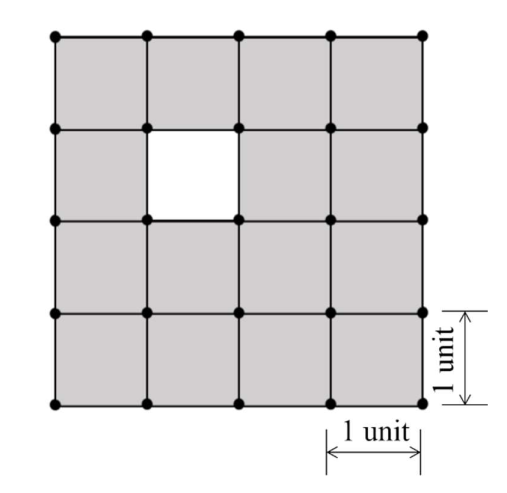
\includegraphics[width=0.2\columnwidth]{fig1}
	\caption{}
	\label{fig:placeholder}
	\end{figure}


What is the maximum number of squares without a ``hole in the interior'' that can be formed within the $4 \times 4$ grid using the unit squares as building blocks?  

\medskip

\begin{multicols}{4}
  
\begin{enumerate}
	\item [(A)] 15
	\item [(B)] 20
	\item [(C)] 21
	\item [(D)] 26
\end{enumerate}

\end{multicols}


\hfill(GATE NM 2022)






\item  An art gallery engages a security guard to ensure that the items displayed are protected. The diagram below represents the plan of the gallery where the boundary walls are opaque. The location the security guard posted is identified such that all the inner space (shaded region in the plan) of the gallery is within the line of sight of the security guard.  

If the security guard does not move around the posted location and has a $360^\circ$ view, which one of the following correctly represents the set of \textbf{ALL} possible locations among the locations P, Q, R and S, where the security guard can be posted to watch over the entire inner space of the gallery.  

\begin{figure}[h]
	\centering
	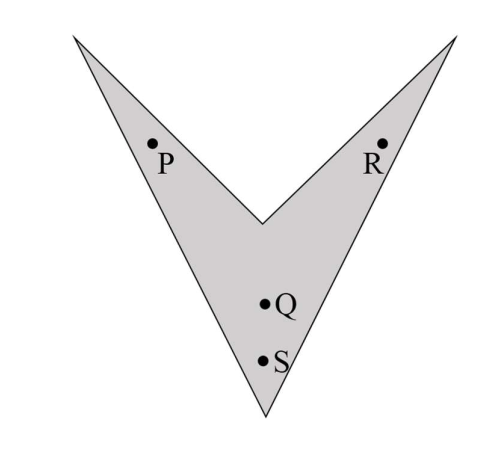
\includegraphics[width=0.3\columnwidth]{fig2}
	\caption{}
	\label{fig:placeholder}
\end{figure}

\begin{multicols}{4}

\begin{enumerate}
    \item[(A)] P and Q
    \item[(B)] Q
    \item[(C)] Q and S
    \item[(D)] R and S
\end{enumerate}

\end{multicols}

\hfill(GATE NM 2022)





\item  Mosquitoes pose a threat to human health. Controlling mosquitoes using chemicals may have undesired consequences. In Florida, authorities have used genetically modified mosquitoes to control the overall mosquito population. It remains to be seen if this novel approach has unforeseen consequences.  

Which one of the following is the correct logical inference based on the information in the above passage?  

\begin{enumerate}
    \item[(A)] Using chemicals to kill mosquitoes is better than using genetically modified mosquitoes because genetic engineering is dangerous
    \item[(B)] Using genetically modified mosquitoes is better than using chemicals to kill mosquitoes because they do not have any side effects
    \item[(C)] Both using genetically modified mosquitoes and chemicals have undesired consequences and can be dangerous
    \item[(D)] Using chemicals to kill mosquitoes may have undesired consequences but it is not clear if using genetically modified mosquitoes has any negative consequence
\end{enumerate}

\hfill(GATE NM 2022)



\item  Consider the following inequalities:  
$	
    \text{(i)} \quad   2x - 1 > 7 \\
 \text{(ii)} \quad   2x - 9 < 1
$

Which one of the following expressions below satisfies the above two inequalities? 

\begin{multicols}{2}

\begin{enumerate}
    \item[(A)] $x \leq -4$
    \item[(B)] $-4 < x \leq 4$
    \item[(C)] $4 < x < 5$
    \item[(D)] $x \geq 5$
\end{enumerate}

\end{multicols}

\hfill(GATE NM 2022)



\item  Four points $P(0, 1)$, $Q(0, -3)$, $R(-2, -1)$, and $S(2, -1)$ represent the vertices of a quadrilateral.  

What is the area enclosed by the quadrilateral? 

\begin{multicols}{4}

\begin{enumerate}
    \item[(A)] $4$
    \item[(B)] $4\sqrt{2}$
    \item[(C)] $8$
    \item[(D)] $8\sqrt{2}$
\end{enumerate}

\end{multicols}

\hfill(GATE NM 2022)






\item  In a class of five students P, Q, R, S and T, only one student is known to have copied in the exam. The disciplinary committee has investigated the situation and recorded the statements from the students as given below.  

{Statement of P:} R has copied in the exam.  

{Statement of Q:} S has copied in the exam.  

{Statement of R:} P did not copy in the exam.  

{Statement of S:} Only one of us is telling the truth.  

{Statement of T:} R is telling the truth.  

The investigating team had authentic information that S never lies.  

Based on the information given above, the person who has copied in the exam is  

\begin{multicols}{4}

\begin{enumerate}
    \item[(A)] R
    \item[(B)] P
    \item[(C)] Q
    \item[(D)] T
\end{enumerate}

\end{multicols}

\hfill(GATE NM 2022)








\item  Consider the following square with the four corners and the center marked as $P$, $Q$, $R$, $S$ and $T$ respectively.  

Let $X$, $Y$ and $Z$ represent the following operations:  
\begin{itemize}
	\item $X$: rotation of the square by $180{\degree}$ with respect to the S--Q axis.
	\item $Y$: rotation of the square by $180{\degree}$ with respect to the P--R axis.
	\item $Z$: rotation of the square by $90{\degree}$ clockwise with respect to the axis perpendicular, going into the screen and passing through the point $T$.
\end{itemize}

Consider the following three distinct sequences of operation (which are applied in the left to right order):  
$
\text{(1) } XYZZ \quad\quad \text{(2) } XY \quad\quad \text{(3) } ZZZZ
$

Which one of the following statements is correct as per the information provided above?  


\begin{figure}[h]
	\centering
	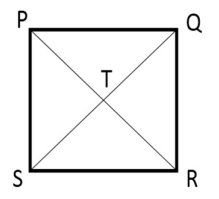
\includegraphics[width=0.2\columnwidth]{fig3}
	\caption{}
	\label{fig:placeholder}
\end{figure}

\begin{enumerate}
    \item[(A)] The sequence of operations (1) and (2) are equivalent
    \item[(B)] The sequence of operations (1) and (3) are equivalent
    \item[(C)] The sequence of operations (2) and (3) are equivalent
    \item[(D)] The sequence of operations (1),(2) and (3) are equivalent
\end{enumerate}

\hfill(GATE NM 2022)








\item  Let $A$ be a real non-zero square matrix of order $n$. If the homogeneous system of linear equations $A x = 0$ has only trivial solution, then

\begin{enumerate}
    \item[(A)] the matrix $A$ is singular
    \item[(B)] the determinant of $A$ is zero
    \item[(C)] $\lambda = 0$ is an eigenvalue of $A$
    \item[(D)] for any $n$-vector $b$, the system of linear equations $A x = b$ has a unique solution
\end{enumerate}

\hfill(GATE NM 2022)






\item  Let $z = x + i y$, where $x$ and $y$ are real numbers. Consider the complex functions:
\begin{align*}
f(z) = (x^2 - y^2) + i\,  2xy
\end{align*}
and
\begin{align*}
g(z) = 2xy + i (x^2 - y^2).
\end{align*}
Then on the complex plane,
\begin{enumerate}
    \item[(A)] $f(z)$ is analytic and $g(z)$ is not analytic
    \item[(B)] both $f(z)$ and $g(z)$ are analytic
    \item[(C)] both $f(z)$ and $g(z)$ are not analytic
    \item[(D)] $f(z)$ is not analytic and $g(z)$ is analytic
\end{enumerate}

\hfill(GATE NM 2022)






\item  If a population has exponential distribution with mean $1$, then its median is

	\begin{multicols}{4}

\begin{enumerate}
    \item[(A)] $e$
    \item[(B)] $1$
    \item[(C)] $\log 2$
    \item[(D)] $\log 3$
\end{enumerate}

	\end{multicols}

\hfill(GATE NM 2022)




\item  Let $\omega_f$ be the excitation frequency of a sinusoidal load and $\omega_n$ be the natural frequency of a single degree of freedom system. Then the dynamic response of the system is highly affected by the stiffness of the system when

	\begin{multicols}{2}

\begin{enumerate}
    \item[(A)] $\omega_f = \omega_n$
    \item[(B)] $0 < \omega_f < \omega_n$
    \item[(C)] $0 < \omega_n < \omega_f$
    \item[(D)] $\omega_f = 0$
\end{enumerate}

	\end{multicols}

\hfill(GATE NM 2022)








\item  A truck loaded with a half-filled water tank is moving at a constant horizontal acceleration $a$. The acceleration due to gravity is $g$. At steady state, the angle $\theta$ made by the free surface with the horizontal plane is

	\begin{multicols}{4}

\begin{enumerate}
    \item[(A)] $\sin^{-1}\!\left(\frac{a}{g}\right)$
    \item[(B)] $\tan^{-1}\!\left(\frac{g}{a}\right)$
    \item[(C)] $\tan^{-1}\!\left(\frac{a}{g}\right)$
    \item[(D)] $\sin^{-1}\!\left(\frac{g}{a}\right)$
\end{enumerate}

	\end{multicols}

\hfill(GATE NM 2022)





\item  Which one of the following combinations of elementary flows will lead to an ideal flow past a deeply submerged circular cylinder with circulation?

\begin{enumerate}
    \item[(A)] Source, sink and uniform flow
    \item[(B)] Doublet, uniform flow and vortex
    \item[(C)] Doublet and vortex
    \item[(D)] Source and uniform flow
\end{enumerate}


\hfill(GATE NM 2022)





\item  A 10000 tonne displacement container ship's main propulsion engine has a brake power equal to $46$ MW  and its service speed is $25$ knots. Considering the engine brake power as double the effective power of the ship, then the ship resistance at the service speed lies in between \_\_\_\_\_  kN.

	\begin{multicols}{2}

\begin{enumerate}
    \item[(A)] 3285 and 3315
    \item[(B)] 6785 and 6815
    \item[(C)] 885 and 915
    \item[(D)] 1785 and 1815
\end{enumerate}

	\end{multicols}

\hfill (GATE NM 2022)







\item  The margin line used for the floodable length calculation of a ship is

\begin{enumerate}
    \item[(A)] 76 mm above the ship's baseline
    \item[(B)] 76 mm inside the zero-buttock line in the profile view of the ship's lines plan
    \item[(C)] a line drawn 76 mm parallel to and below the watertight main deck at side
    \item[(D)] a line drawn 76 mm parallel to and below the watertight main deck along the ship's centerline if the ship has camber
\end{enumerate}

\hfill (GATE NM 2022)





\item  Consider a rectangular box barge of length $80$ m , breadth $20$ m  and depth $15$ m  floating at an even draught of $10$ m . Assume that the heave added mass of the vessel is equal to its mass displacement and the acceleration due to gravity is $9.81  m/s^2 $ . The heave natural period of the vessel lies in between \_\_\_\_\_  s.

	\begin{multicols}{4}

\begin{enumerate}
    \item[(A)] 1 and 5
    \item[(B)] 6 and 10
    \item[(C)] 11 and 15
    \item[(D)] 16 and 20
\end{enumerate}

	\end{multicols}

\hfill(GATE NM 2022)





\item  A $1{:}20$ scaled model of a surface ship is tested in a towing tank. The model is towed at 3 m/s  and drag force measured is $10$N. The velocity of the prototype and the drag force acting on the prototype, respectively, are \_\_\_\_   m/s and \_\_\_\_   kN.

	\begin{multicols}{4}

\begin{enumerate}
    \item[(A)] 60.4 and 80
    \item[(B)] 13.4 and 80
    \item[(C)] 13.4 and 4
    \item[(D)] 60.4 and 4
\end{enumerate}

	\end{multicols}

\hfill(GATE NM 2022)





\item  In a diesel engine, the ignition is initiated by the

	\begin{multicols}{2}

\begin{enumerate}
    \item[(A)] spark
    \item[(B)] preheating of the fuel
    \item[(C)] heating due to the compression of intake air
    \item[(D)] preheating of the intake air
\end{enumerate}

	\end{multicols}

\hfill(GATE NM 2022)



\item  In an internal combustion engine, supercharging is the process of supplying intake air at a pressure

\begin{enumerate}
    \item[(A)] higher than that of the ambient
    \item[(B)] lower than that of the fuel
    \item[(C)] higher than that of the fuel
    \item[(D)] lower than that of the ambient
\end{enumerate}

\hfill(GATE NM 2022)






\item  The most desirable property amongst the following for a lubricating oil is

	\begin{multicols}{2}

\begin{enumerate}
    \item[(A)] high density
    \item[(B)] high dynamic viscosity
    \item[(C)] low density
    \item[(D)] low dynamic viscosity
\end{enumerate}

	\end{multicols}

\hfill(GATE NM 2022)









\item  If
$
\frac{a_0}{2} + \sum_{n=1}^{\infty} a_n \cos(nx)
$
is the Fourier cosine series of the function
\begin{align*}
f(x)=\sin x,\qquad 0<x<\pi,
\end{align*}
then which of the following are TRUE?

\begin{multicols}{4}

\begin{enumerate}
	\item [(A)] $a_0 + a_1 = \dfrac{4}{\pi}$
	\item  [(B)] $a_0 = \dfrac{4}{\pi}$
	\item [(C)]  $a_0 + a_1 = \dfrac{2}{\pi}$
	\item  [(D)] $a_1 = \dfrac{2}{\pi}$
\end{enumerate}

\end{multicols}

\hfill(GATE NM 2022)





\item  A simply supported beam is loaded with a uniformly distributed load (UDL) acting vertically downwards. Which of the following statements are TRUE with regard to strain energy?

\begin{enumerate}
	\item  [(A)] It increases with increase in UDL
	\item  [(B)] It increases with increase in cross-sectional area of the beam
	\item  [(C)] It is independent of the length of the beam
	\item  [(D)] It is dependent on Young's modulus of elasticity
\end{enumerate}

\hfill(GATE NM 2022)







\item  Which of the following flows are represented by the velocity field,  
$
\vec{V} = (x^2 - y^2)\,\hat{i} - 2xy\,\hat{j} \, ?
$

\begin{multicols}{2}

\begin{enumerate}
    \item[(A)] Incompressible flow
    \item[(B)] Compressible flow
    \item[(C)] Irrotational flow
    \item[(D)] Rotational flow
\end{enumerate}

\end{multicols}

\hfill(GATE NM 2022)




\item  If a ship enters shallow water from deep water, maintaining the same speed, then which of the following are TRUE?

	\begin{multicols}{2}

\begin{enumerate}
    \item[(A)] Resistance increases
    \item[(B)] Trim changes
    \item[(C)] Resistance decreases
    \item[(D)] Draught increases
\end{enumerate}

	\end{multicols}

\hfill(GATE NM 2022)






\item  For a rigid vessel at sea, which of the following statements are TRUE?

\begin{enumerate}
    \item[(A)] Static and dynamic environmental loads are dependent on the structural strength of the vessel
    \item[(B)] Static and dynamic environmental loads are NOT dependent on the structural strength of the vessel
    \item[(C)] Static and dynamic environmental loads are dependent on the geometry of the vessel
    \item[(D)] Static and dynamic environmental loads are NOT dependent on the geometry of the vessel
\end{enumerate}

\hfill(GATE NM 2022)




\item  Which of the following are TRUE for pressure, temperature and density of a thermodynamic system?

	\begin{multicols}{2}

\begin{enumerate}
    \item[(A)] path functions
    \item[(B)] point functions
    \item[(C)] inexact differentials
    \item[(D)] exact differentials
\end{enumerate}

	\end{multicols}

\hfill(GATE NM 2022)







\item  Let $ f(x, y, z) = xy + yz + xz . $ If a point $ (0, 0, \lambda) $ lies on the tangent plane to the surface  
$
f(x, y, z) = 3
$
at the point $ (1, 1, 1) $, then the value of $ \lambda $ is \_\_\_\_\_ .

\hfill(GATE NM 2022)







\item  The beam fixed at end $A$ and simply supported at $C$ with a roller is shown in the figure.  
If $B$  is an internal hinge and a concentrated load of $10$ kN is acting at $D$ and a uniformly distributed load (UDL) of $10$ kN/m  is acting on member $AB$, then the magnitude of bending moment at the fixed end $A$ is \_\_\_\_\_\_\_ kNm.

\begin{figure}[h]
	\centering
    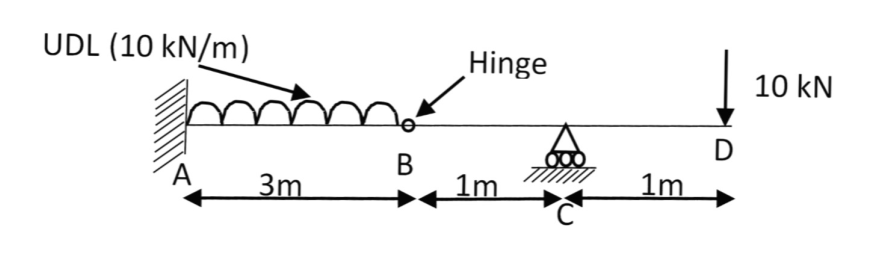
\includegraphics[width=0.3\columnwidth]{fig4}
	\caption{}
	\label{fig:placeholder}
\end{figure}

\hfill(GATE NM 2022)







\item  The laminar and turbulent boundary layer thickness of a flat plate are given by  
$
\frac{5x}{\ \text{Re}_x^{1/2}}
\quad \text{and} \quad
\frac{0.37x}{\ \text{Re}_x^{1/5}},
$
respectively, where $x$ is the distance from the leading edge and $\ \text{Re}_x$ is the Reynolds number at $x$-location.  

The kinematic viscosity of the fluid is $10^{-6}~\ \text{m}^2/\ \text{s}$.  
A $100~\ \text{m}$  long plate is moving at a speed of $10~\ \text{m/s}$.  
The boundary layer thickness at the rear end of the plate is \_\_\_\_\_ m (rounded off to two decimal places).

\hfill(GATE NM 2022)






\item  The diameter and rotating speed of a cargo ship propeller are $7.5$ m  and $120$ RPM , respectively.  
An open water test is to be performed in a towing tank with a propeller model of 300 mm  diameter.  
The corresponding propeller model speed is \_\_\_\_\_ RPM.

\hfill(GATE NM 2022)
















\item  Assume that a ship has length L = 200 m  and operates at a design speed $U = 12$ m/s.  
If in a turning circle maneuver, the ship exhibits a steady turning diameter of $6L$, then the yaw rate of the ship is \_\_\_\_\_ rad/s (correct to two decimal places).

\hfill(GATE NM 2022)









\item  If the maximum static deflection of a shaft is $5$ mm , then the estimated critical speed using Rayleigh--Ritz method is \_\_\_\_\_ RPM  (rounded off to nearest integer).

	\hfill(GATE NM 2022)


\item  The value of the line integral  
\begin{align*}
\oint_C \!\left( -3y \, dx + 3x \, dy + z \, dz \right)
\end{align*}
along the circle $C: x^2 + y^2 = 1, \ z = 1$ oriented in the clockwise sense as seen from the origin, is

\begin{multicols}{4}

\begin{enumerate}
    \item[(A)] $2\pi$
    \item[(B)] $4\pi$
    \item[(C)] $6\pi$
    \item[(D)] $8\pi$
\end{enumerate}

\end{multicols}

\hfill(GATE NM 2022)







\item  A column of height $20$ m  is fixed at both ends.  
If Young's modulus of elasticity is $17 \times 10^{9}$ $ N/m^2 $ and moment of inertia is $3.255 \times  10^{-4}$ $ m^4 $, then the first critical load of buckling of the column lies between \_\_\_\_\_ kN.

\begin{multicols}{4}

\begin{enumerate}
    \item[(A)] 501 and 520
    \item[(B)] 521 and 540
    \item[(C)] 541 and 560
    \item[(D)] 561 and 580
\end{enumerate}

\end{multicols}

\hfill(GATE NM 2022)










\item  In a potential flow field, if the stream function $\psi = x y^2$, then the velocity potential$\phi$ is

	\begin{multicols}{2}

\begin{enumerate}
	\item[(A)] $\frac{x^2 - y^2}{2} $
	\item[(B)] $\frac{x^2 + y^2}{2} $
	\item[(C)] $y(x^2 + \frac{y^2}{3}) $
	\item[(D)] $y(x^2 - \frac{y^2}{3}) $
\end{enumerate}

	\end{multicols}

\hfill(GATE NM 2022)










\item  For a container ship, the propeller open water efficiency, thrust deduction fraction and wake fraction are 0.60, 0.19 and 0.25, respectively.  
If the relative rotative efficiency of the propeller is 1.0, then the hull efficiency and quasi-propulsive efficiency of the propeller, respectively, are

\begin{multicols}{2}

\begin{enumerate}
    \item[(A)] 1.080 and 0.648
    \item[(B)] 0.608 and 0.556
    \item[(C)] 0.926 and 0.648
    \item[(D)] 0.926 and 0.556
\end{enumerate}

\end{multicols}

\hfill(GATE NM 2022)









\item  Consider the wave elevation spectrum $S_{\eta\eta}(\omega)$ as shown in the figure.  
Then, the significant wave height is \_\_\_\_\_ m.

\begin{figure}[h]
    \centering
	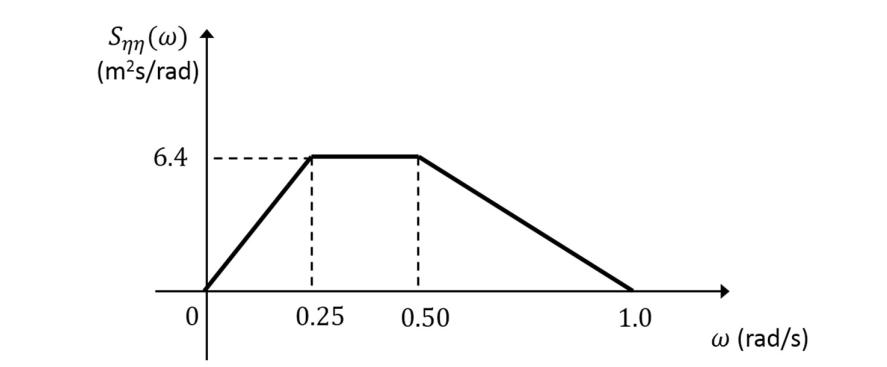
\includegraphics[width=0.3\columnwidth]{fig5}
	\caption{}
	\label{fig:placeholder}
\end{figure}

\begin{multicols}{4}

\begin{enumerate}
    \item[(A)] 2
    \item[(B)] 4
    \item[(C)] 6
    \item[(D)] 8
\end{enumerate}

\end{multicols}

\hfill(GATE NM 2022)











\item  If $\Delta h_m$ and $\Delta h_f$ are the enthalpy drops across the moving and fixed blades of a turbine stage, then the degree of reaction is

	\begin{multicols}{4}

\begin{enumerate}
    \item[(A)] $\dfrac{\Delta h_m}{ \Delta h_f}$
    \item[(B)] $\dfrac{\Delta h_f}{\Delta h_m }$
    \item[(C)] $\dfrac{\Delta h_m }{\Delta h_m + \Delta h_f}$
    \item[(D)] $\dfrac{\Delta h_f }{\Delta h_m + \Delta h_f}$
\end{enumerate}

	\end{multicols}

\hfill(GATE NM 2022)



\item  Let  
$M=
\myvec
{2 & -1 & 1 \\
-1 & 2 & -1 \\
1 & -1 & 2}.
$  

Which of the following are TRUE?

\begin{enumerate}
    \item[(A)] $M$ is singular
    \item[(B)] $M^{-1} = {\frac{1}{4}}M^{2} - {\frac{3}{2}}M + {\frac{9}{4}}I $, where $I$ is the identity matrix of order 3
    \item[(C)] $M$ has three distinct eigenvalues
    \item[(D)] $M$ has three linearly independent eigenvectors
\end{enumerate}

\hfill(GATE NM 2022)












\item  Which of the following statements are TRUE about the assumptions adopted in Euler's column theory?  

\begin{enumerate}
    \item[(A)] Length of the column is very large in comparison to its cross-sectional dimensions
    \item[(B)] Effect of the axial compressive stress is smaller than the effect of bending stress on column buckling
    \item[(C)] Column fails only by transverse loads
    \item[(D)] Column fails only by buckling
\end{enumerate}

\hfill(GATE NM 2022)


\item  An autonomous underwater vehicle is made of a long cylinder with a semi-ellipsoid at the forward end and a hemisphere at the aft end as shown in the figure.  
The origin of the reference frame is located at the centroid of the cylinder.  

The positive $x$, $y$ and $z$ axes, respectively, are pointing towards forward, port and upward directions.  
The surge, sway and heave motions are represented by indices 1--2--3 and roll, pitch and yaw motions are represented by indices 4--5--6, respectively.  

If $A = [A_{ij}]$ is the added mass matrix, then which of the following are NOT zero?

\begin{figure}[h]
	\centering
	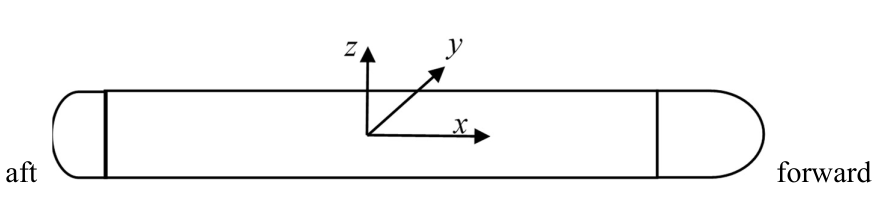
\includegraphics[width=0.3\columnwidth]{fig6}
	\caption{}
	\label{fig:placeholder}
\end{figure}

\begin{multicols}{4}

\begin{enumerate}
    \item[(A)]  $A_{15}$
    \item[(B)]  $A_{35}$
    \item[(C)]  $A_{46}$
    \item[(D)]  $A_{26}$
\end{enumerate}

\end{multicols}

\hfill(GATE NM 2022)



\item  If a ship hull is subdivided into different watertight compartments, which of the following statements are TRUE?

\begin{enumerate}
    \item[(A)] It improves the ship stability in damaged conditions
    \item[(B)] It increases the ship hull strength
    \item[(C)] It reduces the ship intact stability
    \item[(D)] It provides more options to carry different types of cargo
\end{enumerate}

\hfill(GATE NM 2022)









\item  Consider the midship section of a vessel with the centerline (CL) and neutral axis (NA) as shown in the figure.  
Assume that the cross-section is symmetric about the centerline, the plate thickness is uniform throughout the section and $h_1 < h_2$.  

When the vessel is subjected to a vertical bending moment in its upright condition, which of the following statements are TRUE?

\begin{figure}[h]
	\centering
	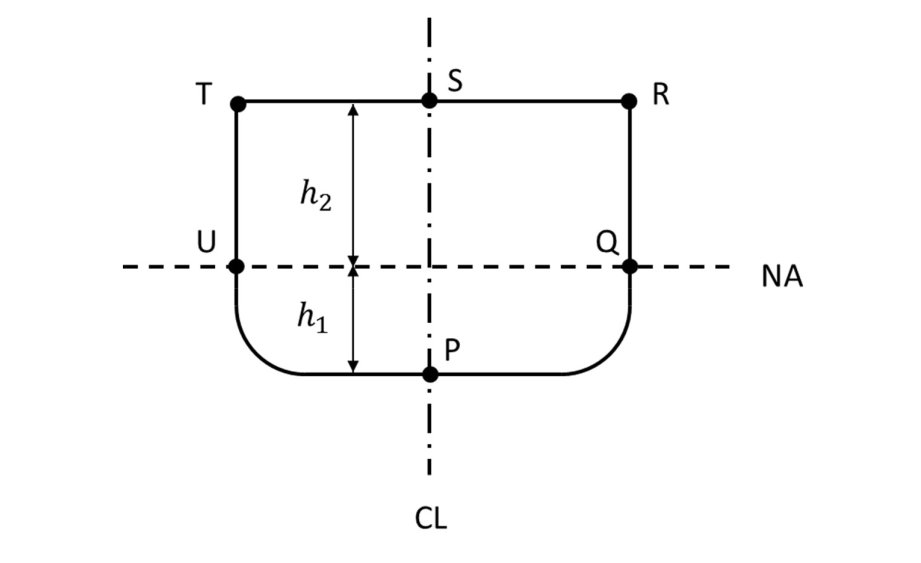
\includegraphics[width=0.3\columnwidth]{fig7}
	\caption{}
	\label{fig:placeholder}
\end{figure}

\begin{enumerate}
    \item[(A)] Magnitude of shear stress is maximum at points P and S
    \item[(B)] Magnitude of shear stress is minimum at points Q and U
    \item[(C)] Magnitude of
	    bending stress is maximum at points S and T
    \item[(D)] Magnitude of bending stress is minimum at points Q and U
\end{enumerate}

\hfill(GATE NM 2022)


\item  For a simple vapour compression refrigeration, which of the following thermodynamic cycles (1--2--3--4) are possible?  
Here, $T$, $P$, $s$ and $h$ indicate temperature, pressure, specific entropy and specific enthalpy, respectively.

\begin{figure}[h]
\centering
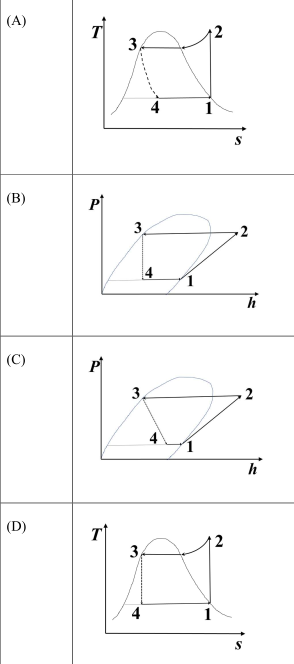
\includegraphics[width=0.2\columnwidth]{fig8}
\caption{}
\label{fig:placeholder}
\end{figure}

\hfill(GATE NM 2022)



\item  Which of the following statements are TRUE for a fluid flow over a deeply submerged body?

\begin{enumerate}
    \item[(A)] D'Alembert's paradox states that a deeply submerged body in a real fluid flow experiences no drag force
    \item[(B)] D'Alembert's paradox states that a deeply submerged body in an ideal fluid flow experiences no drag force
    \item[(C)] The wall shear stress at the point of flow separation on the body is zero
    \item[(D)] Dimples/dentures on a body surface facilitate earlier transition to turbulent flow which delays the boundary layer separation
\end{enumerate}

\hfill(GATE NM 2022)










\item  An Otto cycle has states 1 and 2 at the beginning and the end of the compression stroke, respectively.  
The states 3 and 4 are at the beginning and the end of the expansion stroke, respectively.  

Let the compression ratio of the cycle be $r$, specific heat ratio of air be $\gamma$, specific heat of air at constant volume be $C_v$, and $P$, $v$, and $T$ be pressure, specific volume and temperature of the air, respectively.  
Then, which of the following expressions represent the thermal efficiency of the cycle?

\begin{multicols}{2}

\begin{enumerate}
    \item[(A)] $1 - \dfrac{1}{r^{\gamma - 1}}$
    \item[(B)] $1 - \dfrac{T_3 - T_4}{T_2 - T_1}$
    \item[(C)] $\dfrac{(P_3 v_3 - P_4 v_4) - (P_2 v_2 - P_1 v_1)}{C_v(T_3 - T_2)(\gamma - 1)}$
    \item[(D)] $1 - r^{\gamma - 1}$
\end{enumerate}

\end{multicols}

\hfill(GATE NM 2022)





\item  Let $y(x)$ be the solution of the differential equation  
\begin{align*}
y'' - 4y' - 12y = 3e^{5x}
\end{align*}
satisfying $y(0) = {\frac{18}{7}}$ and $y'(0) = {\frac{-1}{7}}$.  

Then $y(1)$ is \_\_\_\_\_ (rounded off to nearest integer).

\hfill(GATE NM 2022)




\item
We have two coins. One is biased with the probability for head being 1.0 and the other is a fair coin. One coin is chosen at random and is tossed twice. If we obtain head both times, then the probability of the chosen coin being a fair coin is \_\_\_\_\_  (correct to one decimal place).

\hfill(GATE NM 2022)








\item
An element, as shown in the figure, is subjected to stresses $\sigma_x = 500  N/m^2 $, $\sigma_y = 300  N/m^2 $ and $\tau_{xy} = 120  N/m^2 $.  

If $\sigma_1$ and $\sigma_2$ are the principal stresses, then the absolute value of the angle $\phi$ is \_\_\_ degree (rounded off to one decimal place).

\begin{figure}[h]
\centering
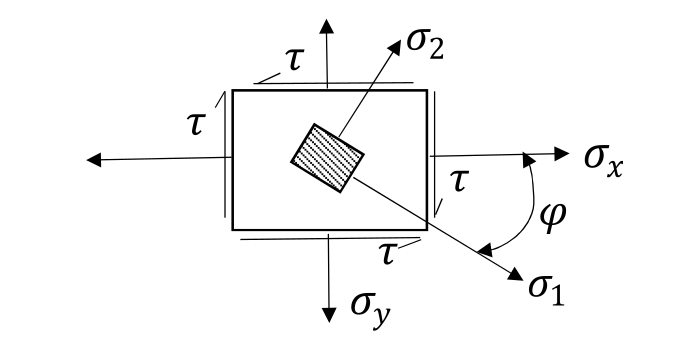
\includegraphics[width=0.3\columnwidth]{fig9}
\caption{}
\label{fig:placeholder}
\end{figure}

\hfill(GATE NM 2022)



\item
An under-damped single degree of freedom system is freely oscillating with an initial amplitude $A$. The initial velocity of the system is zero. After five cycles of oscillation, the amplitude reduces to $A/2$.  

Then the damping ratio of the system is \_\_\_ \% (rounded off to one decimal place) of critical damping.


\hfill(GATE NM 2022)





\item 
A system with two degrees of freedom, as shown in the figure, has masses  
$m_1 = 200$ kg and $m_2 = 100$ kg , and stiffness coefficients  
$k_1 = k_2 = 200$ N/m .  

Then the lowest natural frequency of the system is  
\_\_\_\_  rad/s  (rounded off to one decimal place).


 \begin{figure}[h]
	 \centering
	 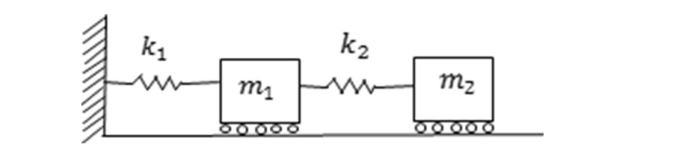
\includegraphics[width=0.3\columnwidth]{fig10}
	 \caption{}
	 \label{fig:placeholder}
 \end{figure}

 \hfill(GATE NM 2022)

\item   
A horizontal cylinder of diameter $1.0$ m  is placed transversely at the aft of a ship and is completely immersed in water.  
The cylinder rotates at $100$ RPM  and the inflow velocity is $10$ m/s . Water density is $1000 kg/m^3 $ .  

Assuming an ideal planar flow, the lift force per unit length acting on the cylinder is  
\_\_\_\_  kN/m (rounded off to one decimal place).


\hfill(GATE NM 2022)



\item  
Consider a steady flow through a horizontal nozzle.  
The nozzle inlet area is $1 m^2 $  and the outlet area is $0.05$ m.  
At the outlet, the flow discharges to atmosphere.  

Assuming the flow to be incompressible and frictionless, and the density of the fluid as  
$1  kg/m^3$, the gauge pressure required at the nozzle inlet to produce an outlet speed  
of $100\ m/s $ is \_\_\_\_\_ $  N/m^2 $ (rounded off to nearest integer).

\hfill(GATE NM 2022)





\item 
A rectangular barge has length $L = 100$ m , breadth $B = 18 $ m  and depth $D = 10$ m .  
It is subdivided transversely into four equal compartments of equal length, with the end compartments loaded fully with oil of density $0.9\ tonne/m^3 $.  
The barge floats in water having a density of $1000  kg/m^3 $.  
If the hull structural weight is ignored, then the transverse metacentric height of the barge is  
\_\_\_\_\_\_  m (correct to two decimal places).

\begin{figure}[h]
\centering
	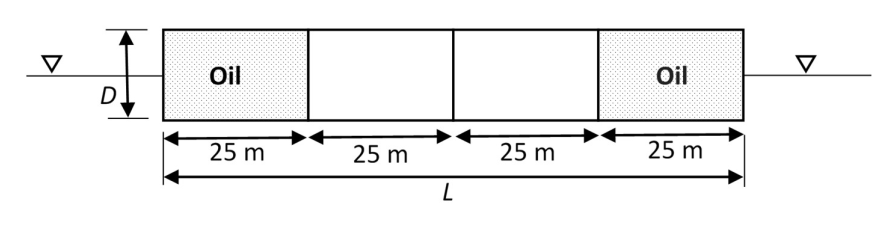
\includegraphics[width=0.3\columnwidth]{fig11}
	\caption{}
	\label{fig:placeholder}

\end{figure}

\hfill(GATE NM 2022)



\item  
A propeller rotating at a speed of $108\ RPM $ behind the ship produces a thrust of  
$720$ kN  with a torque of $700$ kNm, when it travels at a speed of  
$15$ knots .  

In open water, this propeller rotating at the same speed, produces the same thrust at an  
advance speed of $12$ knots , and develops the same torque at an advance speed  
of $12.3$ knots.  

Then, the average of the wake fractions is \_\_\_\_\_\_\_ (correct to two decimal places).


\hfill(GATE NM 2022)






\item  
Consider a point source in a uniform flow of velocity $U = 4$ m/s  along the positive $x$-axis as shown in the figure.  
Assume a two-dimensional steady potential flow.  
The potential due to the point source is given by $\log_e(r)$, where $r^2 = x^2 + y^2$.  

Then the magnitude of the distance $d$ between the point source and the stagnation point is  
\_\_\_\_\_\_ m  (rounded off to two decimal places).


\begin{figure}[h]
	\centering
	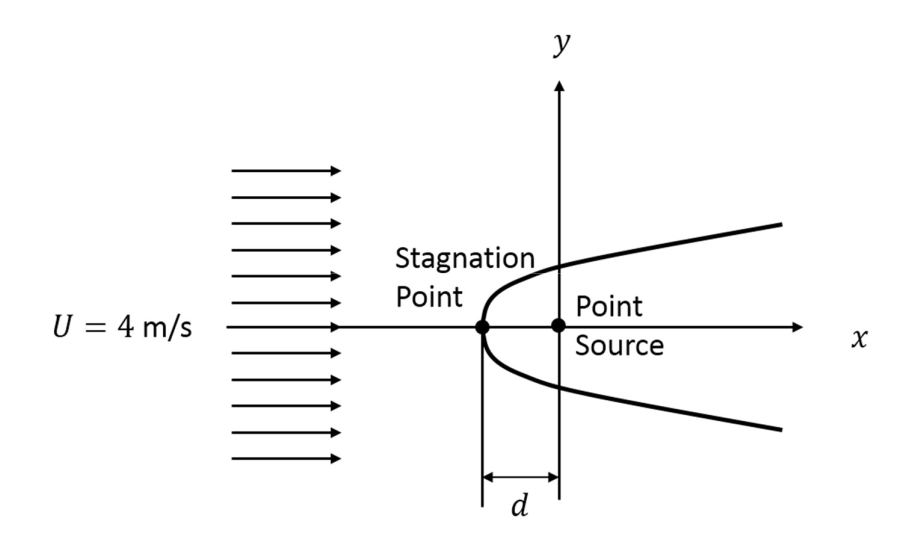
\includegraphics[width=0.3\columnwidth]{fig12}
	\caption{}
	\label{fig:placeholder}
\end{figure}

\hfill(GATE NM 2022)

\item 
Consider a ship with one half of its midship cross-section, as shown in the figure,  
with moulded breadth $B = 30$ m  and moulded depth $D = 9$ m .  

Assume the following:  
- The deck, side shell, and bottom plate have the same thickness.  
- The yield stress of the material is $240$ MPa.  
- The section is subjected to a vertical bending moment of $712.8$ MNm .  
- Ignore the self-moment of inertia of the deck and bottom plating in calculations.  
- The distance of the fiber farthest from the neutral axis can be considered excluding the plate thickness.  

If the maximum bending stress is equal to the yield stress, then the plate thickness is  
\_\_\_\_\_  $\ mm $ (rounded off to one decimal place).


\begin{figure}[h]
	\centering
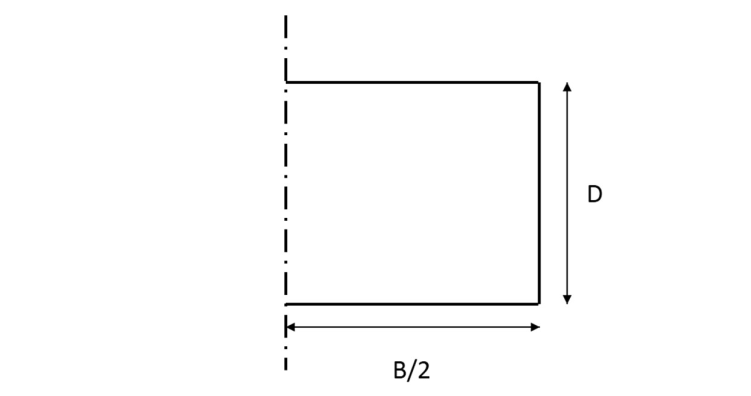
\includegraphics[width=0.3\columnwidth]{fig13}
	\caption{}
	\label{fig:placeholder}
\end{figure}

\hfill(GATE NM 2022)



\item 
Consider a ship  with a forward speed of  
$U = 9.81\ m/s $. A wave is incident at an angle $\beta = 120\degree $  
to the longitudinal axis of the ship, as shown in the figure. Assume acceleration  
due to gravity $g = 9.81\ m/s^2 $.  

If a person onboard the ship observes the encounter period of the incident wave to be  
$4.187\ s $, then the actual period of the wave is  
\_\_\_\_\_ s  (rounded off to one decimal place).

\begin{figure}[h]
	\centering
	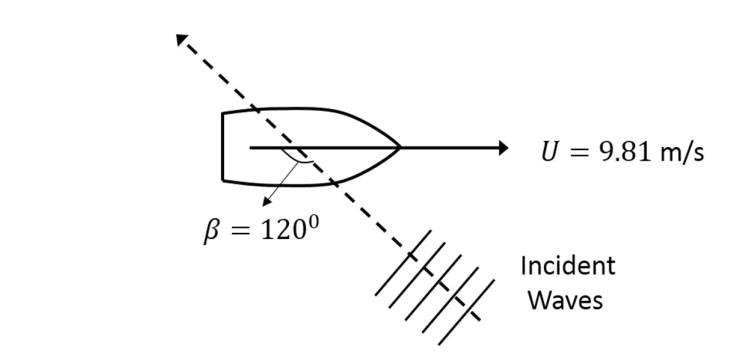
\includegraphics[width=0.3\columnwidth]{fig14}
	\caption{}
	\label{fig:placeholder}
\end{figure}

\hfill(GATE NM 2022)


\item  
An air standard Otto cycle has a compression ratio of 6 and a mean effective pressure of 1000 kPa.  
Assume that  the specific heat ratio $\gamma$ as 1.4 and specific gas constant $R$ as 0.287 kJ/kgK for the air.  
If the pressure and temperature at the beginning of the compression stroke are 100 kPa and 300 K, respectively,  
then the specific work output of the cycle is \_\_\_\_\_ kJ/kg  (rounded off to one decimal place).


\hfill(GATE NM 2022)





\item
If methane (CH$_4$) gas reacts with air at a stoichiometric proportion, then the air-fuel ratio of the combustion process is  
\_\_\_\_ (rounded off to one decimal place).

\hfill(GATE NM 2022)





\item 
In a vapour compression refrigeration cycle using R134 as the refrigerant, the enthalpies are:  
(i) 240 kJ/kg at the beginning of the compression,  
(ii) 275 kJ/kg at the end of the compression, and  
(iii) 96 kJ/kg at the beginning of the throttling.  

Then the coefficient of performance (COP) of the cycle is \_\_\_\_  (rounded off to one decimal place).

\hfill(GATE NM 2022)







\item  
Consider a steady incompressible laminar flow between two parallel long plates separated by a distance  
$h = 1$ m  as shown in the figure.  
The bottom plate is fixed, and the flow is driven by the motion of the upper plate alone.  
No externally imposed pressure exists.  

If the upper plate has a velocity of $U = 10$ m/s , the kinematic viscosity of the fluid is  
$10^{-6}\ m^2/s$, and the density of the fluid is $10^3\ kg/m^3$,  
then the shear stress at the bottom plate is \_\_\_\_  $\ N/m^2  $ (correct to two decimal places).

\begin{figure}[h]
	\centering
	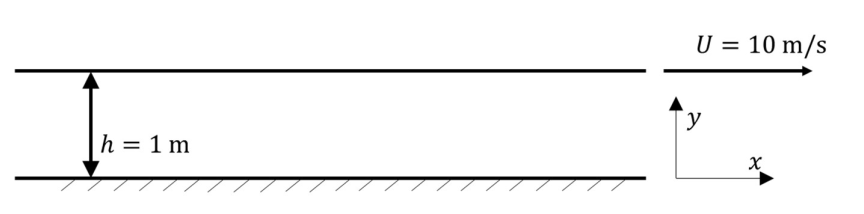
\includegraphics[width=0.5\columnwidth]{fig15}
	\caption{}
	\label{fig:placeholder}
\end{figure}

\hfill(GATE NM 2022)

\begin{tabular}[12pt]{ |c| c| } 
    \hline
    {Group I: Aircraft mode} & {Group II: Property}\\ 
    \hline
    P: Short period mode & 1: Coupled roll-yaw oscillations\\
    \hline 
    Q: Wing rock & 2: Angle of attack remains constant \\
    \hline
    R: Phugoid mode & 3: Roll oscillations \\
    \hline   
    S: Dutch roll & 4: Speed remains constant\\
    \hline
\end{tabular}








\end{enumerate}

\end{document}


































































 



















































































































































